\documentclass[11pt]{article}

% ---------------------------------------------------------------------------
% PODI surrogate report -- OpenFOAM Hackathon Challenge (OFW21), Guimaraes
% Compile with pdflatex (twice). Figures live in ./figures/.
% ---------------------------------------------------------------------------
\usepackage[a4paper,margin=2.3cm]{geometry}
\usepackage{graphicx}
\usepackage{booktabs}
\usepackage{amsmath,amssymb}
\usepackage{xcolor}
\usepackage{caption}
\usepackage{array}
\usepackage[hidelinks]{hyperref}

\graphicspath{{figures/}}
\definecolor{good}{RGB}{20,120,40}
\newcommand{\imp}[1]{{\color{good}#1}}
\captionsetup{font=small,labelfont=bf}
\setlength{\parindent}{0pt}
\setlength{\parskip}{5pt}

\title{\vspace{-1.2cm}\textbf{A PODI Surrogate for Full-Day Air-Quality Prediction\\ in Guimar\~aes}}
\author{OpenFOAM Hackathon Challenge --- OFW21 \\
\normalsize Reduced-order modelling of CO and NO\textsubscript{x} dispersion across mobility scenarios}
\date{}

\begin{document}
\maketitle
\vspace{-0.8cm}

% ===========================================================================
\section*{Executive summary}
A linear \emph{Proper Orthogonal Decomposition with Interpolation} (PODI) surrogate was built
from the CFD dispersion snapshots so that the pollutant field for \emph{any} hour and mobility
scenario can be reconstructed in milliseconds instead of a full parallel dispersion solve. The
surrogate was trained on 40 converged fields (4 scenarios $\times$ 10 representative hours) per
pollutant on the 48.4-million-cell Guimar\~aes mesh, and validated on a held-out 25\% of the
cases (test relative-$L_2$ of 0.33, parity $R^2=0.96$ for both CO and NO\textsubscript{x}). It was
then used to predict the concentration at the four sensitive receptors over the \emph{full
24-hour day} for all four scenarios --- the daily cycle that the direct CFD study could only
sample at ten hours. The predictions reproduce the expected physics exactly (electrification
scales every receptor by $-20\%$ / $-40\%$) and recover the location-dependent benefit of the
Metro Bus (strongest at the Public Hospital), at roughly five orders of magnitude lower cost per
evaluation.

% ===========================================================================
\section{Motivation}
A single dispersion field requires a parallel \texttt{scalarTransportFoam} solve on the frozen
hourly flow. Covering the full day for every scenario and pollutant is
$24\times4\times2=192$ solves on a 48.4M-cell mesh; for that reason the direct CFD assessment
restricted itself to ten representative hours. PODI removes this bottleneck: the converged fields
already computed are treated as \emph{snapshots}, and a low-dimensional linear model is fitted
that maps the physical inputs (wind and emission) to the field. Once trained, it evaluates in
milliseconds, so the entire 24-hour cycle at the receptors --- the natural extension identified as
future work in the CFD report --- becomes trivial to produce, and any intermediate emission level
can be queried without a new simulation.

% ===========================================================================
\section{Input data and labelling}
\textbf{Snapshots.} The training data are the converged dispersion fields of the reference case
and the three mobility scenarios, exported from the decomposed OpenFOAM cases with
\texttt{foamToNumpy} (one \texttt{.npy} per processor plus cell volumes). Each snapshot is the
volumetric concentration field over all $N_{\text{cells}}=48\,358\,418$ cells at one hour, for one
pollutant (\texttt{T\_CO} for CO, \texttt{T\_NOx} for NO\textsubscript{x}). Ten representative
hours (a maximin selection over wind speed/direction and emission totals) are used for each
scenario, giving $n=40$ snapshots per pollutant.

\textbf{Labels.} Every snapshot is tagged with the four physical parameters that generated it,
$p=(u,v,G,L)$: the two horizontal wind-inlet components $(u,v)$ of that hour, a global emission
scale $G\in[0,1]$ applied to all road segments, and a local emission scale $L\in[0,1]$ applied to
the N101/Metro-Bus corridor segments (\texttt{road\_ids\_reduction.txt}). Cases are named
\texttt{<tag>\_h<N>} (e.g.\ \texttt{full\_h0}, \texttt{S1\_h3}), and the labels are stored in
\texttt{parameters.csv}. The scenario-to-control mapping is:

\begin{table}[h]
\centering
\begin{tabular}{@{}llcc@{}}
\toprule
Scenario & Definition & $G$ (global) & $L$ (N101) \\
\midrule
Reference        & Provided traffic                         & 1.0 & 1.0 \\
S1               & 20\% of gas vehicles $\rightarrow$ EV    & 0.8 & 1.0 \\
S2               & 40\% of gas vehicles $\rightarrow$ EV    & 0.6 & 1.0 \\
S3               & Metro Bus ($-50\%$ on N101 corridor)     & 1.0 & 0.5 \\
\bottomrule
\end{tabular}
\caption{Mobility scenarios expressed as emission-scale labels for the surrogate.}
\end{table}

\textbf{Split.} The 40 cases are divided 75/25 into training and test sets, stratified by the
$(G,L)$ scenario so that every scenario appears in both sets: 32 training and 8 test snapshots,
with the same split (fixed seed) shared by both pollutants.

% ===========================================================================
\section{Method and ansatz function}
\textbf{Magnitude--shape decoupling.} Across the sampled cases the field magnitude spans about
$50\times$, because concentration dilutes roughly as $1/|U|$ with wind speed and scales exactly
with emission. A single linear map cannot hold that range, so each snapshot $x_c$ is split into a
scalar volume-weighted magnitude and a unit-norm \emph{shape},
\begin{equation}
s_c = \lVert x_c\rVert_V = \sqrt{x_c^{\!\top} V x_c}, \qquad
\hat{x}_c = x_c / s_c , \qquad V=\mathrm{diag}(\text{cell volumes}).
\end{equation}

\textbf{POD by the method of snapshots.} POD is applied to the shapes through the small
volume-weighted Gram matrix $S_{ij}=\hat{x}_i^{\!\top} V \hat{x}_j$ ($n\times n$), whose
eigen-decomposition yields the modes $\phi_k$ and singular values $\sigma_k$ without ever forming
the $N_{\text{cells}}\times r$ basis explicitly --- essential at 48M cells.

\textbf{Ansatz.} For a new parameter vector $p=(u,v,G,L)$ the field is reconstructed as
\begin{equation}
\boxed{\;x(p) \;=\; m(p)\,\Big[\,\bar{x} \;+\; \sum_{k=1}^{r}\phi_k\,a_k(p)\Big]\;}
\end{equation}
i.e.\ a scalar \emph{magnitude} $m(p)$ multiplying a \emph{shape} that is the POD mean $\bar{x}$
plus a linear combination of $r$ modes. The modal coefficients are an affine map of standardized,
physics-augmented parameters,
\begin{equation}
a_k(p) = w_{k0} + \sum_j w_{kj}\,\tilde{f}_j(p),\qquad
f(p)=\big(u,\,v,\,G,\,L,\,|U|,\,1/|U|,\,G/|U|\big),\quad |U|=\sqrt{u^2+v^2},
\end{equation}
fitted by least squares on the training coefficients. The magnitude is a multiplicative
(log-linear) model
\begin{equation}
\log m(p) = \log G \;+\; b_0 \;+\; b_L\log L \;+\; g(u,v),
\end{equation}
where $g(u,v)$ is a thin-plate-spline RBF interpolation of the wind dependence (the same hourly
winds recur across scenarios). The explicit $\log G$ term encodes the exact physical fact that,
for a frozen flow, passive-scalar dispersion is \emph{linear in emission}. Five modes ($r=5$) were
retained (Section~4).

% ===========================================================================
\section{Validation study}
The number of modes was chosen by sweeping $r$ and comparing the training leave-one-out error with
the held-out test error, both computed entirely in Gram space (no field reconstruction).
Figure~\ref{fig:modes} shows the error plateauing by $r=5$; further modes do not improve the test
error, so $r=5$ is kept as the parsimonious choice. Table~\ref{tab:val} summarises the accuracy.

\begin{table}[h]
\centering
\begin{tabular}{@{}lccc@{}}
\toprule
Pollutant & Modes $r$ & Test relative-$L_2$ & Parity $R^2$ \\
\midrule
CO  (\texttt{T\_CO})  & 5 & 0.332 & 0.963 \\
NO\textsubscript{x} (\texttt{T\_NOx}) & 5 & 0.325 & 0.963 \\
\bottomrule
\end{tabular}
\caption{Surrogate accuracy on the 8-case held-out test set (train-LOO $\approx 0.34$--$0.36$).}
\label{tab:val}
\end{table}

\begin{figure}[h]
\centering
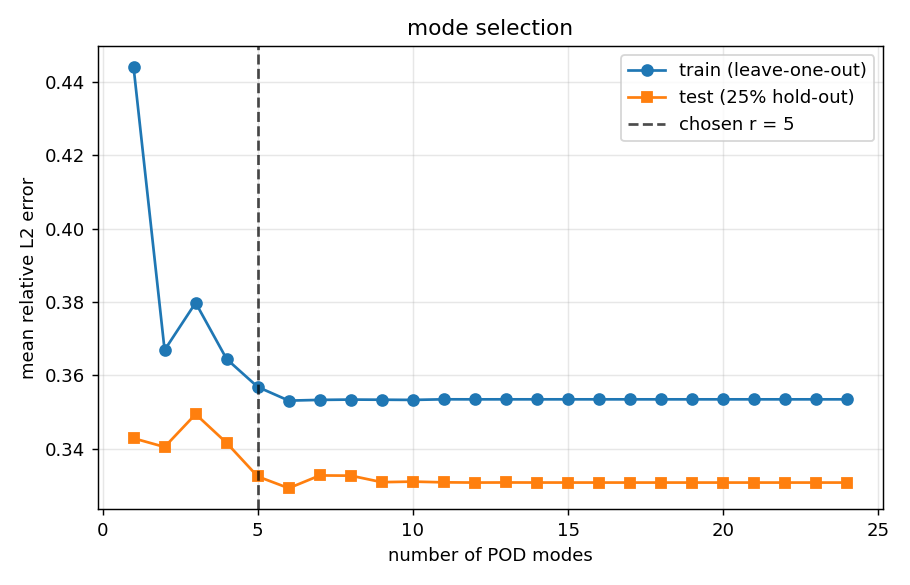
\includegraphics[width=0.48\textwidth]{co_mode_selection.png}\hfill
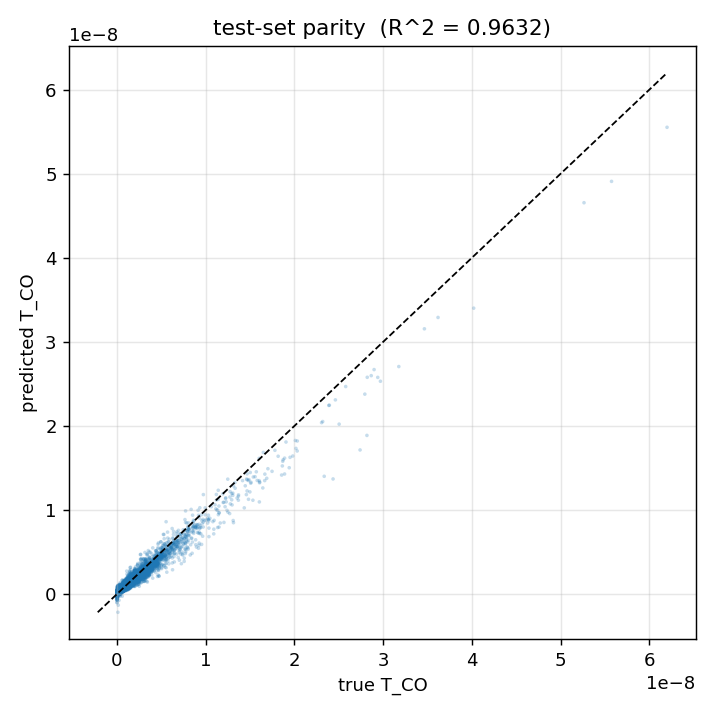
\includegraphics[width=0.48\textwidth]{co_parity.png}
\caption{Left: mode selection --- mean relative-$L_2$ vs number of POD modes (train leave-one-out
and 25\% hold-out), chosen $r=5$ marked. Right: test-set parity of predicted vs true cell values
(CO); NO\textsubscript{x} is equivalent ($R^2=0.963$).}
\label{fig:modes}
\end{figure}

\textbf{Independent physical cross-check.} Beyond the statistical split, the surrogate was verified
against a directly-simulated field. For the reference case at 07:00, the predicted CO field matches
the CFD field with a volume-weighted relative-$L_2$ of 0.13, and the area-averaged concentration at
the Public Hospital receptor is $1.52\times10^{-9}$ vs the simulated $1.61\times10^{-9}$
(kg\,m$^{-3}$), a $\sim6\%$ agreement --- confirming that the reconstruction is faithful at the
receptor scale, which is what the assessment ultimately reports.

% ===========================================================================
\section{Prediction results}
The trained surrogate was evaluated at all 24 hourly wind states for the four scenarios and both
pollutants, and the reconstructed fields were sampled at the four ROI receptor surfaces with the
same \texttt{surfaceFieldValue} function objects as the CFD workflow. This yields the full daily
concentration profile at each receptor (Figures~\ref{fig:co-day}--\ref{fig:nox-day}); the
day-averaged and peak values are given in Tables~\ref{tab:co}--\ref{tab:nox}.

\begin{table}[h]
\centering
\begin{tabular}{@{}lccccc@{}}
\toprule
\multicolumn{6}{c}{\textbf{CO} --- daily-mean concentration ($\mu$g\,m$^{-3}$), change vs Reference} \\
\midrule
Receptor & Reference & S1 & S2 & S3 & 24h peak (Ref) \\
\midrule
Public Hospital       & 3.68 & 2.94 \imp{($-20.1\%$)} & 2.20 \imp{($-40.2\%$)} & 2.58 \imp{($-30.0\%$)} & 9.54 \\
Francisco de Holanda  & 2.04 & 1.63 \imp{($-20.0\%$)} & 1.22 \imp{($-40.0\%$)} & 1.71 \imp{($-15.9\%$)} & 5.28 \\
Martins Sarmento      & 3.60 & 2.88 \imp{($-20.0\%$)} & 2.16 \imp{($-39.9\%$)} & 3.04 \imp{($-15.4\%$)} & 9.56 \\
Santos Sim\~oes       & 4.34 & 3.47 \imp{($-19.9\%$)} & 2.61 \imp{($-39.9\%$)} & 3.86 \imp{($-11.0\%$)} & 11.66 \\
\bottomrule
\end{tabular}
\caption{CO daily statistics over the full 24-hour cycle (surrogate prediction).}
\label{tab:co}
\end{table}

\begin{table}[h]
\centering
\begin{tabular}{@{}lccccc@{}}
\toprule
\multicolumn{6}{c}{\textbf{NO\textsubscript{x}} --- daily-mean concentration ($\mu$g\,m$^{-3}$), change vs Reference} \\
\midrule
Receptor & Reference & S1 & S2 & S3 & 24h peak (Ref) \\
\midrule
Public Hospital       & 4.98 & 3.98 \imp{($-20.0\%$)} & 2.99 \imp{($-40.0\%$)} & 3.96 \imp{($-20.4\%$)} & 12.15 \\
Francisco de Holanda  & 2.87 & 2.30 \imp{($-20.0\%$)} & 1.72 \imp{($-40.0\%$)} & 2.38 \imp{($-17.0\%$)} & 6.80 \\
Martins Sarmento      & 5.35 & 4.28 \imp{($-20.0\%$)} & 3.21 \imp{($-40.0\%$)} & 4.45 \imp{($-16.9\%$)} & 13.00 \\
Santos Sim\~oes       & 6.39 & 5.12 \imp{($-20.0\%$)} & 3.84 \imp{($-40.0\%$)} & 5.47 \imp{($-14.5\%$)} & 15.47 \\
\bottomrule
\end{tabular}
\caption{NO\textsubscript{x} daily statistics over the full 24-hour cycle (surrogate prediction).}
\label{tab:nox}
\end{table}

\begin{figure}[h]
\centering
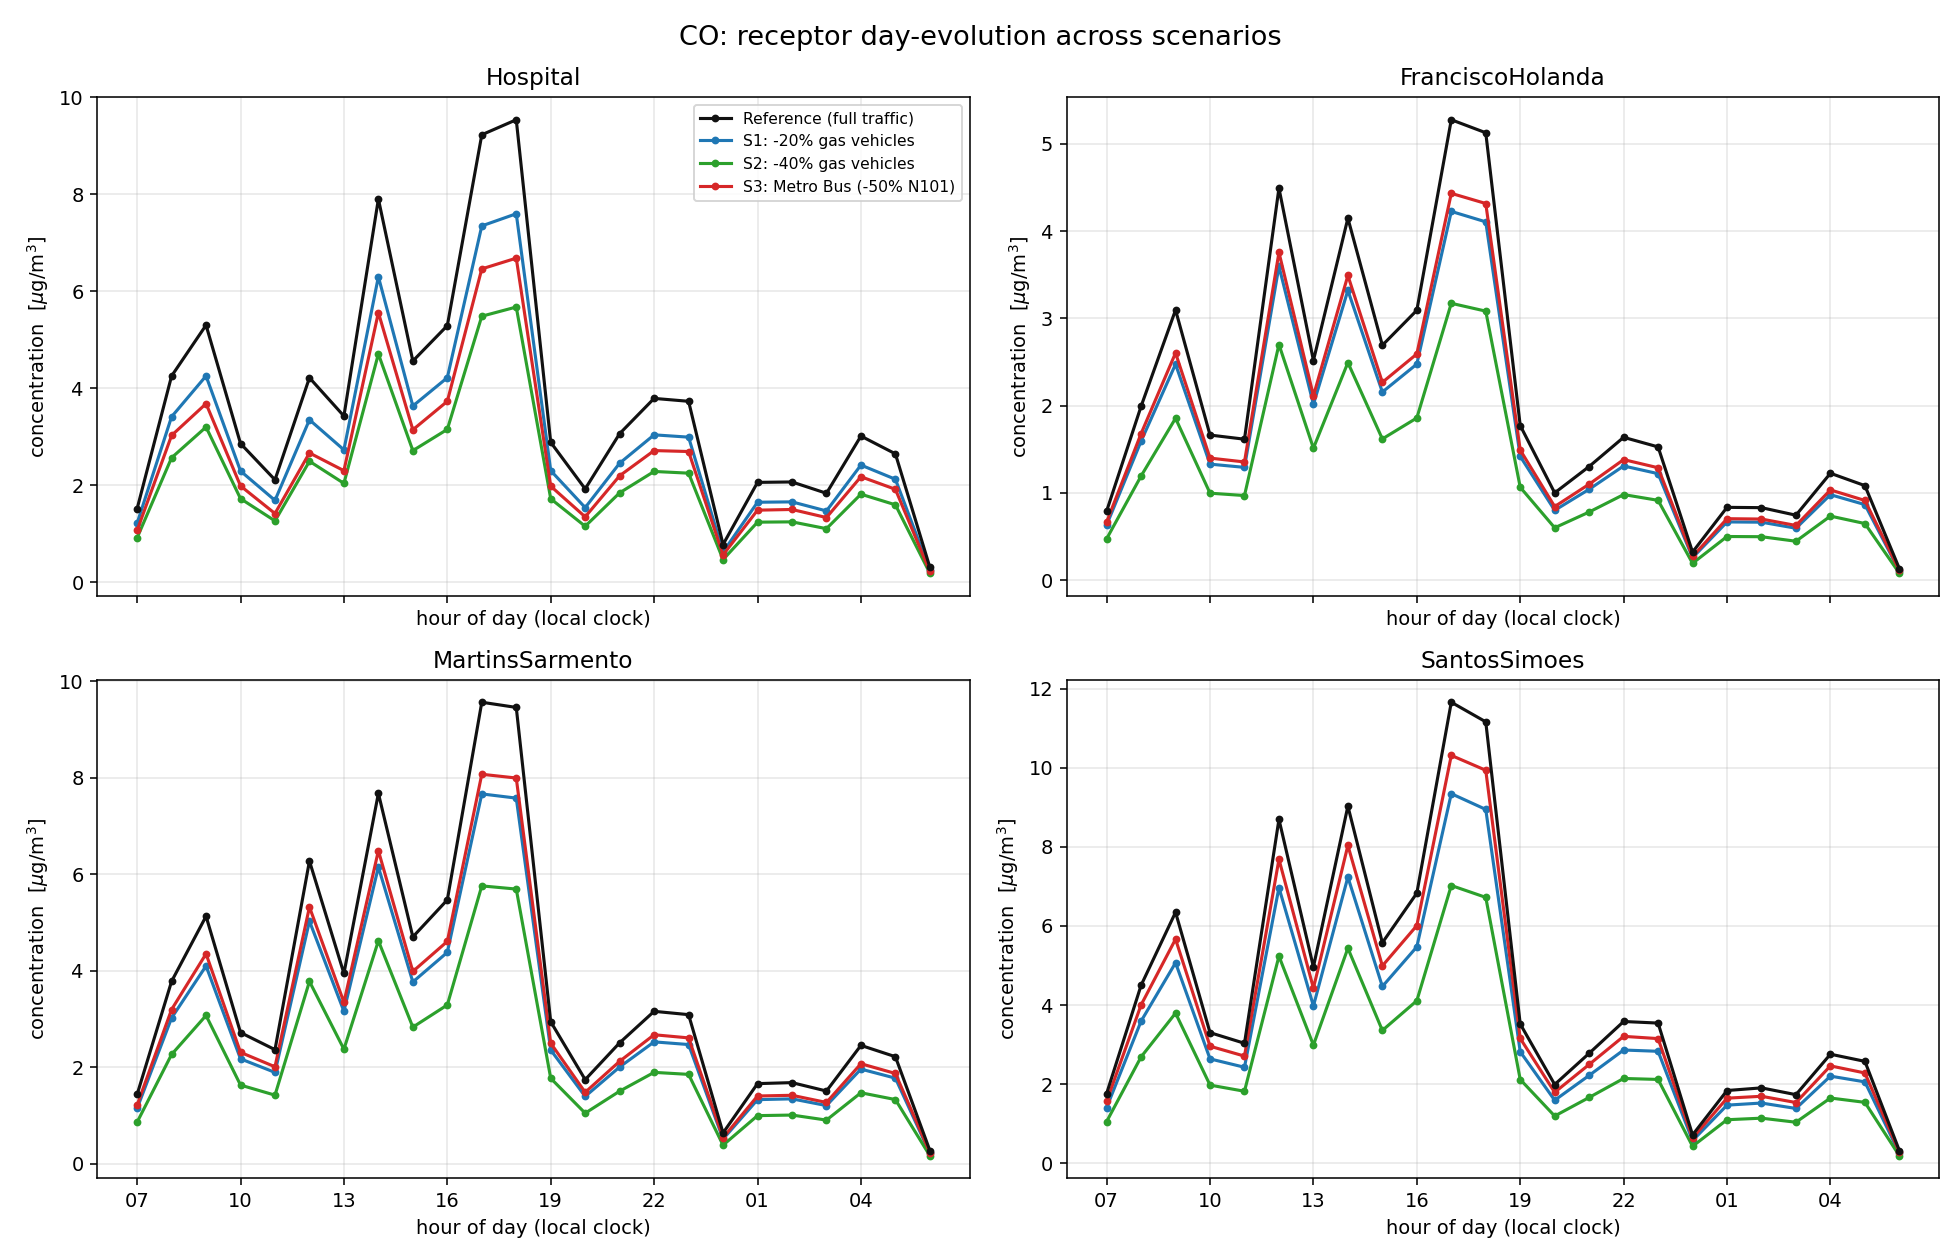
\includegraphics[width=\textwidth]{co_overview.png}
\caption{CO day-evolution at the four receptors: concentration vs hour of day (07:00 $\to$ 06:00),
one curve per scenario. Electrification (S1/S2) lowers every site uniformly; the Metro Bus (S3)
acts most strongly at the Public Hospital.}
\label{fig:co-day}
\end{figure}

\begin{figure}[h]
\centering
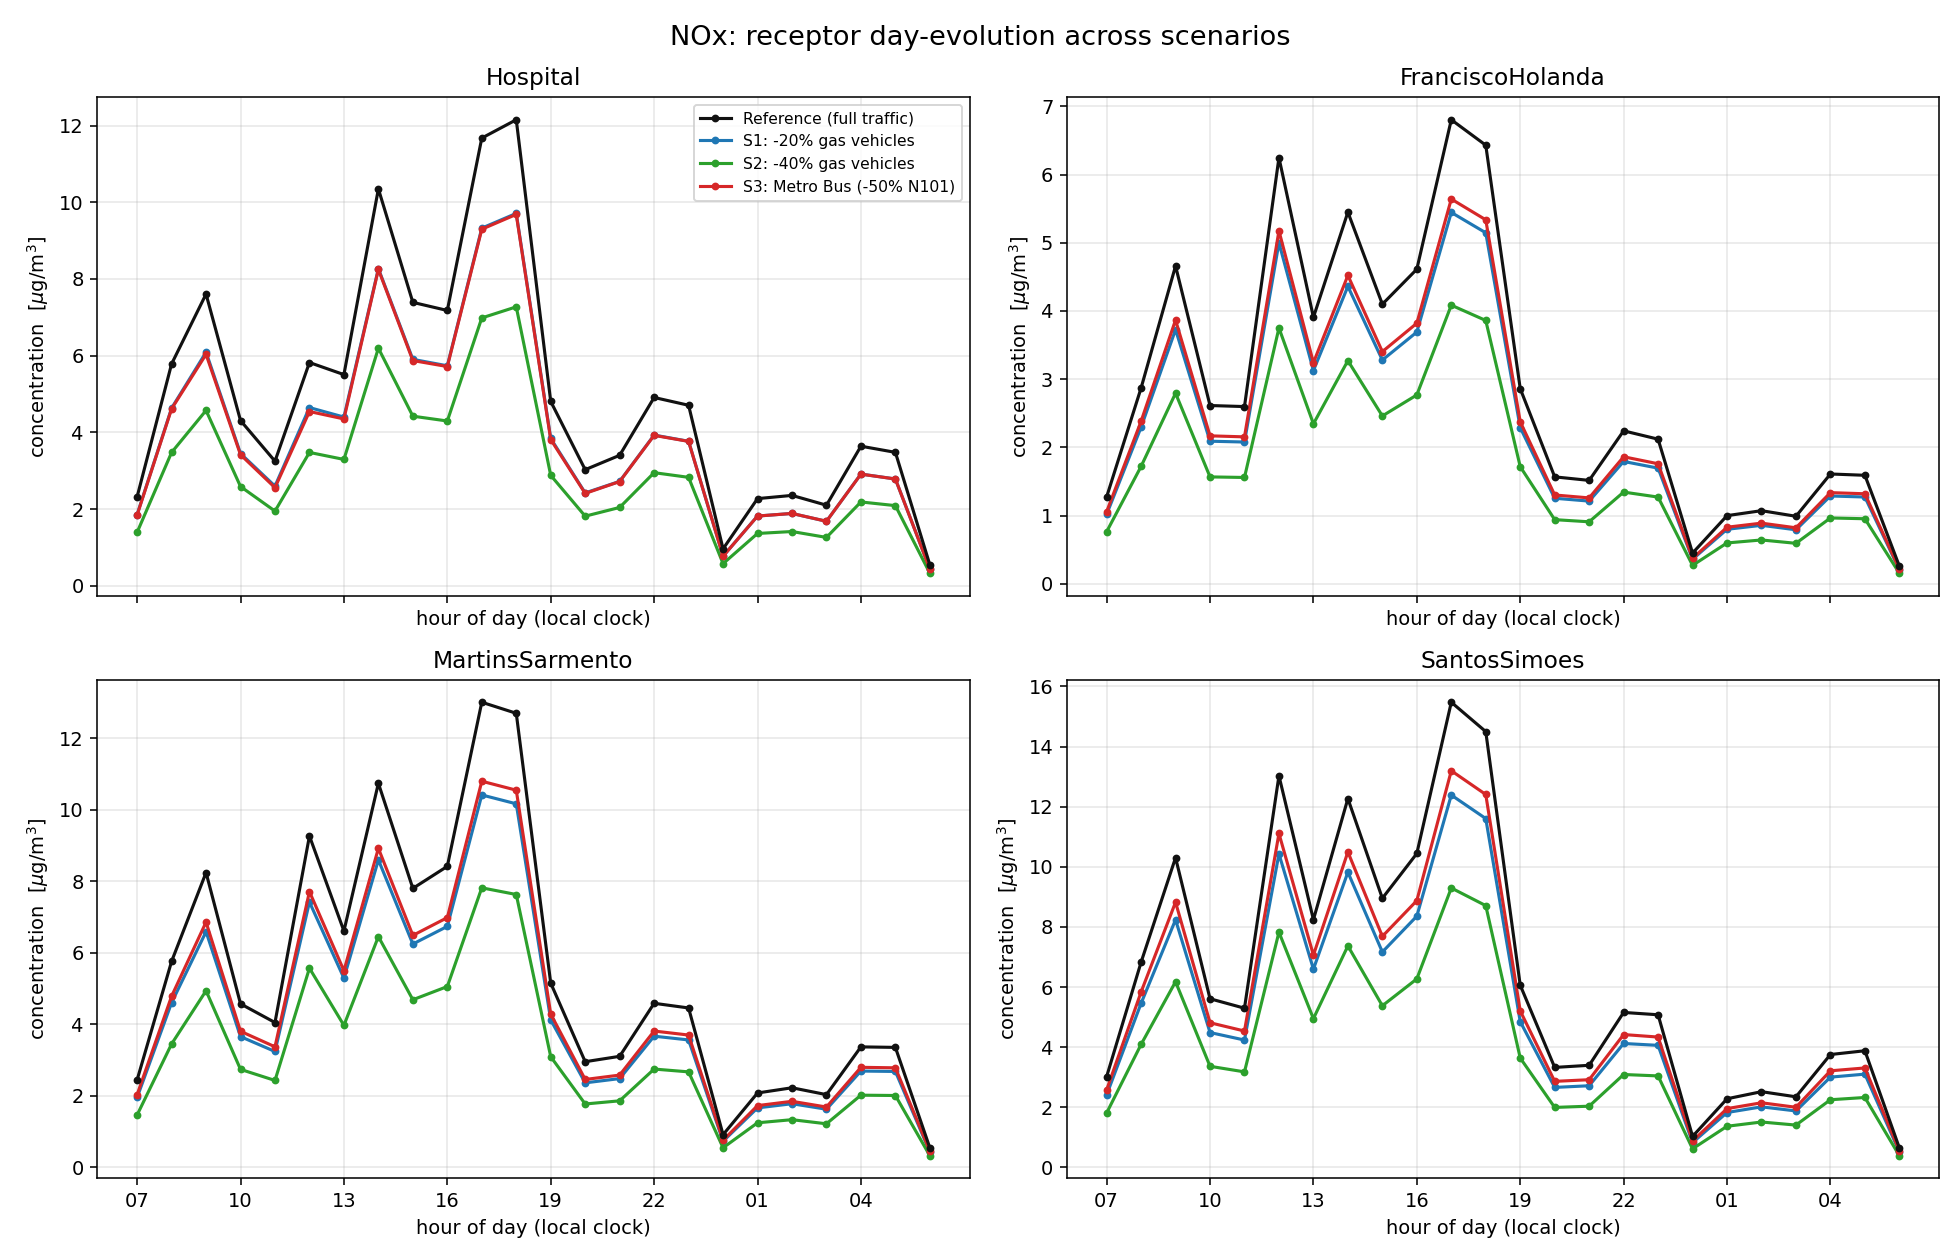
\includegraphics[width=\textwidth]{nox_overview.png}
\caption{NO\textsubscript{x} day-evolution at the four receptors. Same qualitative structure as CO;
NO\textsubscript{x} is the pollutant of interest, with the highest exposure at Santos Sim\~oes.}
\label{fig:nox-day}
\end{figure}

\textbf{Findings.}
(i) Fleet electrification scales every receptor by exactly $-20\%$ (S1) and $-40\%$ (S2) for both
pollutants, at all hours. This is the physically correct response --- dispersion is linear in
emission for a frozen flow --- and serves as a consistency check that the surrogate respects the
emission physics rather than merely interpolating.
(ii) The Metro Bus (S3) is spatially selective: it delivers the largest benefit at the Public
Hospital ($-30\%$ CO, $-20\%$ NO\textsubscript{x} on the daily mean), which sits next to the
reduced corridor, while the off-corridor receptors improve far less --- least of all Santos
Sim\~oes ($-11\%$ CO, $-15\%$ NO\textsubscript{x}), the most-exposed site at baseline.
(iii) Exposure follows the daily wind cycle, peaking in the low-wind evening and midday hours; the
peak concentrations (Tables~\ref{tab:co}--\ref{tab:nox}) are roughly $2$--$3\times$ the daily mean.

% ===========================================================================
\section{Conclusions and future work}
The PODI surrogate provides the quantitative, per-receptor air-quality assessment required by the
challenge, and extends it to the complete 24-hour day for all four scenarios --- something
infeasible by direct simulation within the available budget. The conclusions mirror and refine the
direct CFD study: broad fleet electrification (S2) is the strongest uniform measure
($-40\%$ everywhere); the Metro Bus is the most effective \emph{local} measure for the Public
Hospital and the central corridor but does little for Santos Sim\~oes. No single measure is best
everywhere, so a combined Metro-Bus-plus-electrification strategy would give the most uniform
city-wide improvement; if one site must be prioritised, the bus protects the Hospital while
electrification is needed for Santos Sim\~oes.

Because each surrogate evaluation is essentially free, the natural continuations are:
(a) daily-aggregated \emph{exposure} metrics and threshold-exceedance counts over the true 24-hour
cycle rather than a sampled subset; (b) a combined EV\,+\,Metro-Bus scenario and a continuous sweep
of the reduction level (any $G,L$), which the surrogate can produce without new CFD;
(c) reconstruction of full spatial concentration maps (not just receptors) for the whole day;
(d) reducing the surrogate error by enriching the snapshot set with more hours and by testing a
nonlinear coefficient model; and (e) assessing the influence of the computational domain (a larger
domain with a porous vegetation canopy) by retraining on those snapshots. The exported models
(\texttt{model\_CO.pkl}, \texttt{model\_NOx.pkl}) and the prediction/post-processing pipeline are
provided so that any of these can be run directly.

\end{document}
